\documentclass[10pt]{beamer}
\usetheme[
%%% options passed to the outer theme
%    hidetitle,           % hide the (short) title in the sidebar
%    hideauthor,          % hide the (short) author in the sidebar
%    hideinstitute,       % hide the (short) institute in the bottom of the sidebar
%    shownavsym,          % show the navigation symbols
%    width=2cm,           % width of the sidebar (default is 2 cm)
%    hideothersubsections,% hide all subsections but the subsections in the current section
%    hideallsubsections,  % hide all subsections
    left               % right of left position of sidebar (default is right)
%%% options passed to the color theme
%    lightheaderbg,       % use a light header background
  ]{AAUsidebar}

% If you want to change the colors of the various elements in the theme, edit and uncomment the following lines
% Change the bar and sidebar colors:
%\setbeamercolor{AAUsidebar}{fg=red!20,bg=red}
%\setbeamercolor{sidebar}{bg=red!20}
% Change the color of the structural elements:
%\setbeamercolor{structure}{fg=red}
% Change the frame title text color:
%\setbeamercolor{frametitle}{fg=blue}
% Change the normal text color background:
%\setbeamercolor{normal text}{bg=gray!10}
% ... and you can of course change a lot more - see the beamer user manual.

\definecolor{AAUblue1}{RGB}{ 33, 26, 82}
\definecolor{AAUblue2}{RGB}{ 89, 79,191}
\definecolor{AAUgrey1}{RGB}{ 84, 97,110}
\definecolor{AAUgrey2}{RGB}{104,119,132}
\definecolor{AAUgrey3}{RGB}{162,172,182}
\definecolor{AAUgrey4}{RGB}{222,223,226}
\definecolor{AAUgreen}{RGB}{157,187, 29}
\definecolor{AAUteal} {RGB}{ 94,150,149}
\definecolor{AAUred}  {RGB}{223,103, 82}

\usepackage{blkarray}

\usepackage[utf8]{inputenc}
\usepackage[english]{babel}
\usepackage[T1]{fontenc}
% Or whatever. Note that the encoding and the font should match. If T1
% does not look nice, try deleting the line with the fontenc.
\usepackage{helvet}
\usepackage{tikz}                  % drawing vector graphics
\usepackage{circuitikz}            % drawing circuits
\usepackage{mathtools}
%laplace
\usepackage{mathrsfs}
\usepackage{siunitx}    % si-units
\usepackage{amssymb}

%Bibliography
\usepackage[square]{natbib}

\usepackage{tikz}
\usepackage{circuitikz}
\usepackage{graphicx}
\usepackage{caption}
\usepackage{physics}
\usepackage{subcaption}
\usepackage{stackengine}
\usepackage{media9}
\usepackage{multimedia}
\mathtoolsset{showonlyrefs}

\usetikzlibrary{arrows.meta}
\usetikzlibrary{positioning,calc}
\usetikzlibrary{intersections}
\usetikzlibrary{shapes.misc}
\tikzset{>={Latex[width=1mm,length=1.2mm]},
  Speaker/.pic={
    \filldraw[fill=gray!40,pic actions] 
    (-15pt,0) -- 
      coordinate[midway] (-front) 
    (15pt,0) -- 
    ++([shift={(-6pt,8pt)}]0pt,0pt) coordinate (aux1) -- 
    ++(-18pt,0) coordinate (aux2) 
    -- cycle 
    (aux1) -- ++(0,6pt) -- coordinate[midway] (-back) ++(-18pt,0) -- (aux2);
  },cross/.style={cross out, draw=black, minimum size=2*(#1-\pgflinewidth), inner sep=0pt, outer sep=0pt},cross/.default={1pt},
  Box/.pic={
  \draw (0,0) to (0.5,0) to (0.5,-1) to (0.5,-1) to (-.5,-1) to (-.5,0) to (0,0);
  },
  Sbox/.pic={
  \draw (0,0) to (0,0.5) to (1.5,0.5) to (1.5,-0.5) to (0,-0.5) to (0,0);
  },
  Vbox/.pic={
  \draw (0,0) to (1.5,0) to (1.5,-1) to (-1.5,-1) to (-1.5,0) to (0,0);
  },
  variables/.pic={
  \draw (0,0) to (0,0.5) to (1.5,0.5) to (1.5,-0.5) to (0,-0.5) to (0,0);
  \draw (0,0) to (1.5,0);
  },
  pics/microphone/.style={code={ 
        \draw[black, line width=.2em, rounded corners=1.7ex] 
            (-.85em,4.5ex) -- (-.85em,2ex) -- (.85em,2ex) -- (.85em,4.5ex);
        \fill[black] 
            (-.6em,5ex) to[rounded corners=1.2ex]  
            (-.6em,2.5ex) to[rounded corners=1.2ex] (.6em,2.5ex)
            -- (.6em,5ex) to[rounded corners=.2ex] ++(-.85em,0) to[rounded corners=.2ex] ++(0,.35ex) -- ++(.85em,0)  
            -- (.6em,5.5ex) to[rounded corners=.2ex] ++(-.85em,0) to[rounded corners=.2ex] ++(0,.35ex) -- ++(.85em,0)
            -- (.6em,6ex) to[rounded corners=.2ex] ++(-.85em,0) to[rounded corners=.2ex] ++(0,.35ex) -- ++(.85em,0)
            -- (.6em,6.5ex) to[rounded corners=.2ex] ++(-.85em,0) to[rounded corners=.2ex] ++(0,.35ex) -- ++(.85em,0)
            to[rounded corners=1.2ex]
            (.6em,8ex) to[rounded corners=1.2ex]
            (-.6em,8ex) to[rounded corners=1.2ex] cycle; 
        \fill[black] (-.1em,1.8ex) rectangle (.1em,.5ex);
        \fill[black] (-.5em,.5ex) rectangle (.5em,0);
    }}}

% colored hyperlinks
\newcommand{\chref}[2]{%
  \href{#1}{{\usebeamercolor[bg]{AAUsidebar}#2}}%
}
\tikzstyle{point} = [fill,shape=circle,minimum size=3pt,inner sep=0pt]
\tikzstyle{edge} = [fill=white,midway,inner sep=1pt]



\title[CSB]% optional, use only with long paper titles
{Eksamensopgave 1}

\subtitle{Computerstøttede beregninger}  % could also be a conference name

\date{9. Juni 2020}

\author[Gruppe B303c] % optional, use only with lots of authors
{
	Daniel Bursac Hasanovic     \\
	Jens Koldkur				\\
	Jonas Bach Christensen		\\
	Julie Havbo Lund			\\
	Mads Bjerregaard Kjær		\\
	Mathias Gammelgaard			\\
	Rasmus Jespersgaard
}
% - Give the names in the same order as they appear in the paper.
% - Use the \inst{?} command only if the authors have different
%   affiliation. See the beamer manual for an example

\institute[
%  {\includegraphics[scale=0.2]{aau_segl}}\\ %insert a company, department or university logo
%  Dept.\ of Mathematical Sciences\\
%  Skjernvej 4A\\
%  DK-9220 Aalborg Ø
] % optional - is placed in the bottom of the sidebar on every slide
{% is placed on the title page
%  Dept.\ of Mathematical Sciences\\
%  Skjernvej 4A\\
%  DK-9220 Aalborg Ø
  
  %there must be an empty line above this line - otherwise some unwanted space is added between the university and the country (I do not know why;( )
}


% specify a logo on the titlepage (you can specify additional logos an include them in 
% institute command below
\pgfdeclareimage[height=1.5cm]{titlepagelogo}{AAUgraphics/aau_logo_new} % placed on the title page
%\pgfdeclareimage[height=1.5cm]{titlepagelogo2}{graphics/aau_logo_new} % placed on the title page
\titlegraphic{% is placed on the bottom of the title page
  \pgfuseimage{titlepagelogo}
%  \hspace{1cm}\pgfuseimage{titlepagelogo2}
}

% Sets
\newcommand{\N}{\mathbb{N}}  % natural numbers
\newcommand{\Z}{\mathbb{Z}}  % integers
\newcommand{\Q}{\mathbb{Q}}  % rational numbers
\newcommand{\R}{\mathbb{R}}  % real numbers
\newcommand{\C}{\mathbb{C}}  % complex numbers
\newcommand{\I}{\mathbb{I}}  % imaginary numbers
\renewcommand{\b}[1]{\mathbf{#1}}
\renewcommand{\L}{\mathcal{L}}
\newcommand{\U}{\mathcal{U}}
\newcommand{\Y}{\mathcal{Y}}
\newcommand{\B}{\mathcal{B}}

% Semantics
\let\cross=\times
\let\times=\cdot
\newcommand{\euler}{e}%\mathfrak{e}}
\renewcommand{\exp}[1]{\euler^{#1}}
\renewcommand{\matrix}[1]{\begin{bmatrix}#1\end{bmatrix}}
\newcommand{\amatrix}[2]{\left[\begin{array}{@{}*{#1}{c}|c@{}}#2\end{array}\right]}
\renewcommand{\vec}[1]{\mathrm{\mathbf{#1}}}
\newcommand{\transpose}{^\intercal}
% \newcommand{\dotproduct}{\boldsymbol{\cdot}}
\newcommand{\dotp}{\dotproduct}
\newcommand{\directsum}{\oplus}
\newcommand{\cardinality}[1]{\mathit{card}\bigl({#1}\bigr)}
\newcommand\oast{\stackMath\mathbin{\stackinset{c}{0ex}{c}{0ex}{\ast}{\bigcirc}}}

% Other operators and concepts
\newcommand{\bigO}{\mathcal{O}}                                             % big O
\renewcommand\qedsymbol{$\blacksquare$}                                     % use black square as QED
\DeclarePairedDelimiterXPP{\laplace}[1]{\mathscr{L}}{\{}{\}}{}{#1}          % Laplace transform
\DeclarePairedDelimiterXPP{\invlaplace}[1]{\mathscr{L}^{-1}}{\{}{\}}{}{#1}  % Inverse laplace transform
\DeclarePairedDelimiterXPP{\fourier}[1]{\mathscr{F}}{\{}{\}}{}{#1}          % Fourier transform
\DeclarePairedDelimiterXPP{\invfourier}[1]{\mathscr{F}^{-1}}{\{}{\}}{}{#1}  % Inverse fourier transform

\begin{document}
% the titlepage
{\aauwavesbg%
\begin{frame}[plain,noframenumbering] % the plain option removes the sidebar and header from the title page
  \titlepage
\end{frame}}
%%%%%%%%%%%%%%%%

% TOC
\begin{frame}{Disposition}{}
\tableofcontents
\end{frame}
%%%%%%%%%%%%%%%%

\section{Del 1: Kvadraturregler}
\begin{frame}
\centering
\Huge
Del 1: \\
Kvadraturregler
\end{frame}
%
<<<<<<< HEAD
\begin{frame}
\frametitle{Overskrift}
\begin{itemize}
\item Fisk
\end{itemize}
\end{frame}
=======
%\begin{frame}
%\frametitle{Overskrift}
%\begin{itemize}
%\item Fisk
%\end{itemize}
%\end{frame}
>>>>>>> ce9832f84e1a1054fb7719448950ef3cbf59438d
%%
\begin{frame}
\frametitle{Grafer med forskellige $h_0$}
\begin{minipage}[t]{0.49\textwidth}
$$h_0=10$$ 
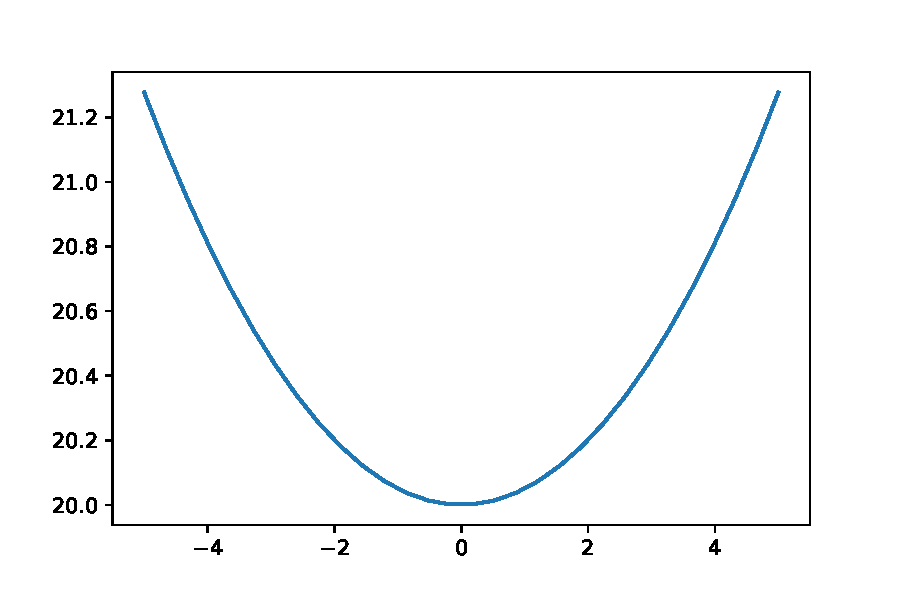
\includegraphics[scale=0.3]{img/fig1}
\end{minipage}
\begin{minipage}[t]{0.49\textwidth}
$$h_0=20$$ 
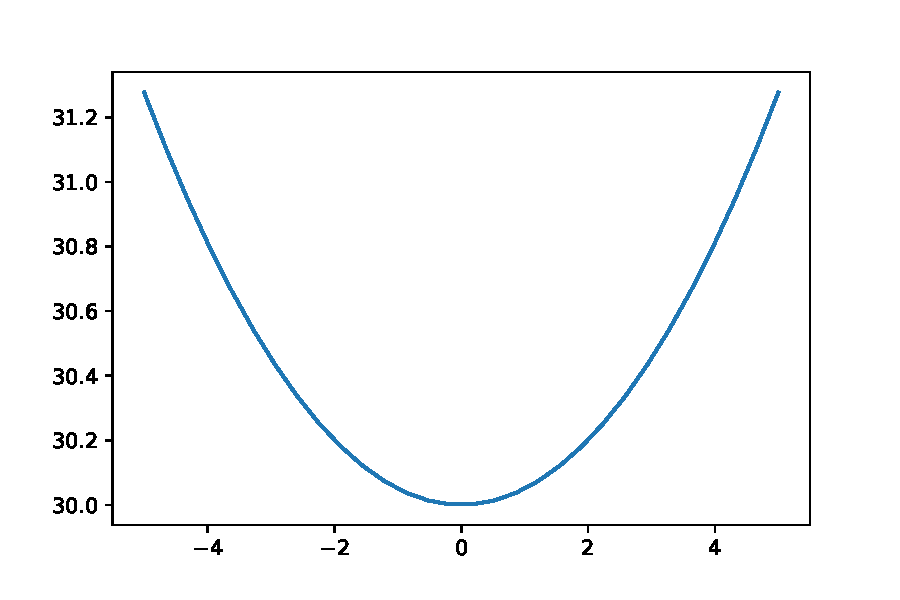
\includegraphics[scale=0.3]{img/fig2}
\end{minipage}
\end{frame}
%
\begin{frame}
\frametitle{Grafer med forskellige $\lambda$}
\begin{minipage}[t]{0.49\textwidth}
$$\lambda=2$$
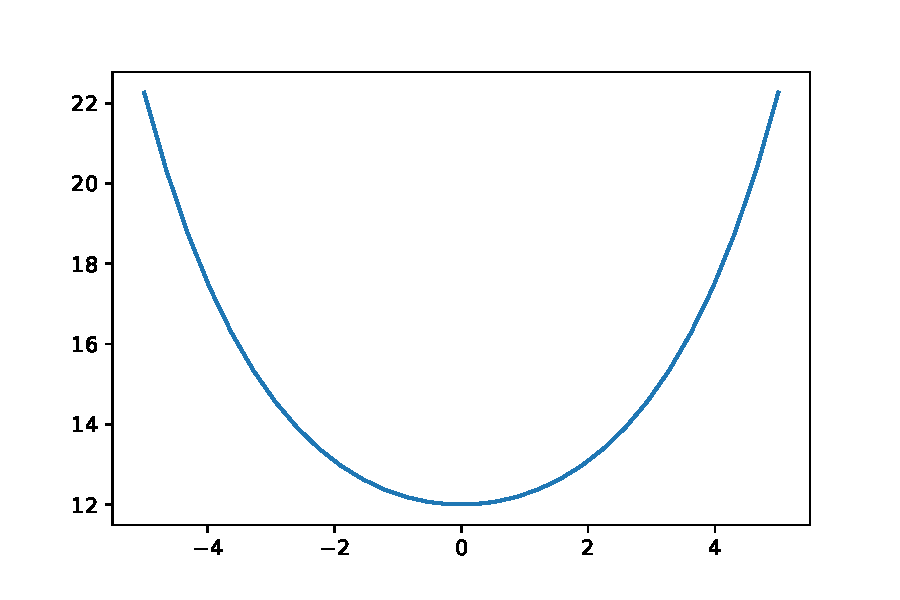
\includegraphics[scale=0.3]{img/fig3}
\end{minipage}
\begin{minipage}[t]{0.49\textwidth}
$$\lambda=1$$
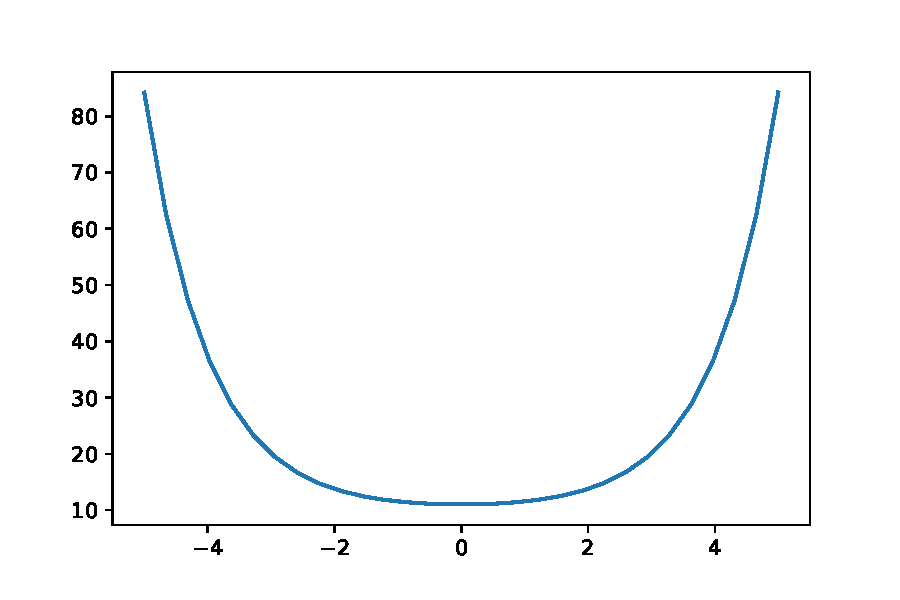
\includegraphics[scale=0.3]{img/fig4}
\end{minipage}
%
\end{frame}




\begin{frame}{Opgave 2: Sammensat kvadraturregel}
    Forklar idéen i en sammensat kvadraturregel. Udled den sammensatte kvadraturregel
    $T_N$.
\end{frame}

\begin{frame}{Sammensat kvadraturregel}
    Ideen ved en sammensat kvadraturregel er, at man tager sit interval fra a til b og inddeler i ækvidistante inddelinger, hvor $x_0$ angiver a, og $x_n$ angiver b og så gælder der ydermere følgende
    \begin{align*}
    a = x_0 < x_1 < … x_{n-1} < x_n = b
    \end{align*}
    $h$ angiver længden intervallerne mellem fx $x_0$ og $x_1$ , og er givet ved $\frac{b-a}{n}$, som betyder, at intervallet derfor inddeles i $n$ såkaldte delintervaller eller underinddelinger. 
    Ideen er så for en sådanne sammensatte kvadraturregel, at der kan anvendes midtpunkt-, trapez- og Simpsons regel på hver af de mindre delintervaller fremfor hele intervallet fra a til b. 
\end{frame}


\begin{frame}{Sammensat kvadraturregel}
    For at udlede den sammensatte kvadraturregel $T_N$ for et integrale, hvor intervallet opdeles i underinddelinger beskrives i følgende
    Trapez-reglen er som sagt, som følger
    \begin{align*}
    T = \frac{h}{2}(f(a)+f(b)),
    \end{align*}
    og ved at omskrive trapez-reglen, så den gælder for to underinddelinger samt indføre notationen for de tilsvarende venstre og højre Riemann summer $h(f(a)+f(a+h)$ og $h(f(a+h)+f(b))$, så får man følgende 
    \begin{align*}
    T_2=\frac{h}{2}(f(a)+f(a+h))+\frac{h}{2}(f(a+h)+f(b)= \frac{h}{2}(f(a)+2f(a+h)+f(b),
    \end{align*}
    hvor $h=\frac{b-a}{2}$.
\end{frame}


\begin{frame}{Sammensat kvadraturregel}
    Bemærk her, at man har evalueringer i det to endepunkter a og b, samt 2 gange evaluering i de indre punkter. Dette er givet, da man benytter trapez-reglen fra intervallet $x_0$ til $x_1$ samt fra $x_1$ til $x_2$, som vil sige, at man har en evaluering i punktet $x_1$ to gange, og derfor divideres med $\frac{1}{2}$. Derved er det videre muligt, at opskrive den generelle formel for den sammensatte kvadraturregel $T_n$ givet ved
    \begin{align*}
    T_n = \frac{1}{2}\left (  h\sum_{k=0}^{N-1}f(a+kh)+h\sum_{k=1}^{N}f(a+kh)\right )
    \end{align*}
    som kan reduceres og omskrives til 
    \begin{align*}
    T_n =\frac{h}{2}\left ((f(a)+2\sum_{k=1}^{N-1}f(a+kh)+f(b) \right )
    \end{align*}
\end{frame}

%%%%
% JULIE
%
\subsection{Nulpunktsbestemmelse}
\begin{frame}
\frametitle{Bisektionsmetoden} 
\begin{itemize}
\item $m=\frac{a+b}{2}$ 
\end{itemize}
%
%%%%%%%%%%%%%%%%%%%%%%%%%%%%%%%%
%%% Flot graf alla Julie     %%%
%%%%%%%%%%%%%%%%%%%%%%%%%%%%%%%%
%
\begin{center}
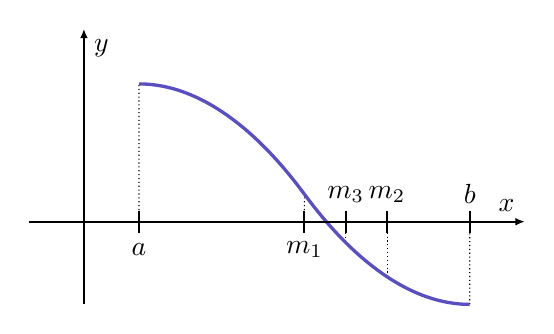
\begin{tikzpicture}[scale=7]
%
% Koordinater 
% ------------------------------------------------------
\coordinate (a) at (0.1,0.5);
\coordinate (b) at (0.4,0.3);
\coordinate (c) at (0.7,0.1);
%
%        
% Streger 
% -------------------------------------------------------
  \draw[densely dotted](0.1,0.25) -- (a);
  \draw[densely dotted](0.4,0.25) -- (b);
  \draw[densely dotted](0.7,0.25) -- (c);
  \draw[densely dotted](0.55,0.23) -- (0.55,0.15);
  \draw[densely dotted](0.475,0.23) -- (0.475,0.21);
  \draw[very thick, color=AAUblue2](a) parabola (b);
  \draw[very thick, color=AAUblue2](b) parabola[bend at end] (c);
  \draw[thick](0.1,0.23) -- (0.1,0.27); % (a)
  \draw[thick](0.7,0.23) -- (0.7,0.27); % (b)
  \draw[thick](0.4,0.23) -- (0.4,0.27); % (m_1)
  \draw[thick](0.55,0.23) -- (0.55,0.27); % (m_2)
  \draw[thick](0.475,0.23) -- (0.475,0.27); % (m_3)
%
%
% Punkt 
% -------------------------------------------------------
\node at (0.1,0.2) (){$a$};
\node at (0.7,0.3) (){$b$};
\node at (0.4,0.2) (){$m_1$};
\node at (0.55,0.3) (){$m_2$};
\node at (0.475,0.3) (){$m_3$};
% 
%
% Koordinatsystemet 
% -------------------------------------------------------
\draw[thick,->] (-0.1,0.25) -- (0.8,0.25) node[anchor=south east]{$x$};
\draw[thick,->] (0,0.1) -- (0,0.6) node[anchor=north west]{$y$};
%
\end{tikzpicture}
\end{center}
\end{frame}
%
\begin{frame}
\frametitle{Integrationsmetoden} 
\begin{itemize}
\item Fixpunktsligning $g(x) = x$
\end{itemize}
%
%%%%%%%%%%%%%%%%%%%%%%%%%%%%%%%%
%%% Flot graf alla Julie     %%%
%%%%%%%%%%%%%%%%%%%%%%%%%%%%%%%%
%
\begin{center}
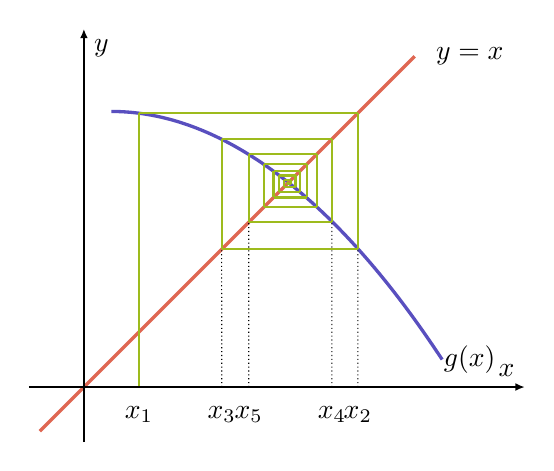
\begin{tikzpicture}[scale=7]
%
% Koordinater 
% ------------------------------------------------------
\coordinate (a) at (0.05,0.5);
\coordinate (b) at (0.65,0.05);
\coordinate (c) at (0.1,0);			% 1
\coordinate (d) at (0.1,0.497);		% 2
\coordinate (e) at (0.497,0.497); 	% 3
\coordinate (f) at (0.497,0.25);
\coordinate (g) at (0.25,0.25);
\coordinate (h) at (0.25,0.45);
\coordinate (i) at (0.45,0.45);
\coordinate (j) at (0.45,0.299);
\coordinate (k) at (0.299,0.299);
\coordinate (l) at (0.299,0.423);
\coordinate (m) at (0.423,0.423);
\coordinate (n) at (0.423,0.327);
\coordinate (o) at (0.327,0.327);
\coordinate (p) at (0.327,0.405);
\coordinate (q) at (0.405,0.405);
\coordinate (r) at (0.405,0.344);
\coordinate (s) at (0.344,0.344);
\coordinate (t) at (0.344,0.392);
\coordinate (u) at (0.392,0.392);
\coordinate (v) at (0.392,0.354);
\coordinate (x) at (0.354,0.354);
\coordinate (y) at (0.354,0.384);
\coordinate (z) at (0.384,0.384);
\coordinate (z1) at (0.384,0.363);
\coordinate (z2) at (0.363,0.363);
\coordinate (z3) at (0.363,0.376);
\coordinate (z4) at (0.376,0.376);
\coordinate (z5) at (0.376,0.368);
\coordinate (z6) at (0.368,0.368);
\coordinate (z7) at (0.372,0.372);
%
%        
% Streger 
% -------------------------------------------------------
  \draw[very thick, color=AAUblue2](a) parabola (b);
  \draw[very thick, color=AAUred] (-0.08,-0.08) -- (0.6,0.6);
  
  \draw[thick, color = AAUgreen](c) -- (d); 
  \draw[thick, color = AAUgreen](d) -- (e); 
  \draw[thick, color = AAUgreen](e) -- (f);
  \draw[thick, color = AAUgreen](f) -- (g);
  \draw[thick, color = AAUgreen](g) -- (h); 
  \draw[thick, color = AAUgreen](h) -- (i); 
  \draw[thick, color = AAUgreen](i) -- (j); 
  \draw[thick, color = AAUgreen](j) -- (k); 
  \draw[thick, color = AAUgreen](k) -- (l); 
  \draw[thick, color = AAUgreen](l) -- (m); 
  \draw[thick, color = AAUgreen](m) -- (n); 
  \draw[thick, color = AAUgreen](n) -- (o); 
  \draw[thick, color = AAUgreen](o) -- (p); 
  \draw[thick, color = AAUgreen](p) -- (q); 
  \draw[thick, color = AAUgreen](q) -- (r); 
  \draw[thick, color = AAUgreen](r) -- (s);
  \draw[thick, color = AAUgreen](s) -- (t); 
  \draw[thick, color = AAUgreen](t) -- (u);   
  \draw[thick, color = AAUgreen](u) -- (v);   
  \draw[thick, color = AAUgreen](v) -- (x);   
  \draw[thick, color = AAUgreen](x) -- (y);   
  \draw[thick, color = AAUgreen](y) -- (z);
  \draw[thick, color = AAUgreen](z) -- (z1);
  \draw[thick, color = AAUgreen](z1) -- (z2);
  \draw[thick, color = AAUgreen](z2) -- (z3);
  \draw[thick, color = AAUgreen](z3) -- (z4);
  \draw[thick, color = AAUgreen](z4) -- (z5);   
  \draw[thick, color = AAUgreen](z5) -- (z6);   
  \draw[thick, color = AAUgreen](z6) -- (z7);       
  
%
% Punkter
% -------------------------------------------------------
%
  \node at (0.7,0.05) (){$g(x)$};
  \node at (0.7,0.6) (){$y=x$};
  
  \node at (0.1,-0.05) (){$x_1$};
  \draw[densely dotted](0.497,0) -- (f);
  \node at (0.497,-0.05) (){$x_2$}; 
  \draw[densely dotted](0.25,0) -- (g);
  \node at (0.25,-0.05) (){$x_3$}; 
  \draw[densely dotted](0.45,0) -- (j);
  \node at (0.45,-0.05) (){$x_4$};
  \draw[densely dotted](0.299,0) -- (k);
  \node at (0.299,-0.05) (){$x_5$};
%  \draw[densely dotted](0.423,0) -- (n);
%  \node at (0.423,-0.05) (){$x_6$};
%  \draw[densely dotted](0.327,0) -- (o);
%  \node at (0.327,-0.05) (){$x_7$};
%
%
% Koordinatsystemet 
% -------------------------------------------------------
\draw[thick,->] (-0.1,0) -- (0.8,0) node[anchor=south east]{$x$};
\draw[thick,->] (0,-0.1) -- (0,0.65) node[anchor=north west]{$y$};
%
\end{tikzpicture}
\end{center}
\end{frame}
%
% MADS 
%
\begin{frame}
\frametitle{Newtons metode}
\begin{itemize}
\item Newtons iterationsformel: 
$$x_{n+1}=x_n- \frac{f(x_n)}{f'(x_n)}$$
\end{itemize}
\begin{center}
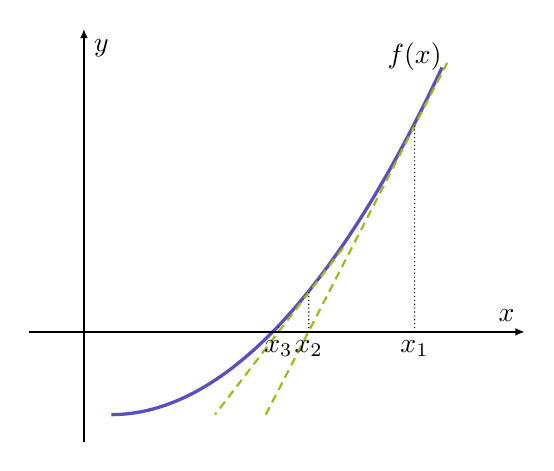
\begin{tikzpicture}[scale=7]
%
% Koordinater 
% ------------------------------------------------------
\coordinate (a) at (0.05,-0.05);
\coordinate (b) at (0.65,0.58);
\coordinate (c) at (0.6,0.48);		% 1
\coordinate (d) at (0.33,-0.05);	% a
\coordinate (e) at (0.66,0.59); 	% b
\coordinate (f) at (0.408,0.173);	% 2
\coordinate (g) at (0.47,0.252);	% a
\coordinate (h) at (0.238,-0.05);	% b
\coordinate (i) at (0.353,0.11);	% 3
\coordinate (j) at (0.32,0.07);		% a
\coordinate (k) at (0.16,-0.05);	% b
\coordinate (l) at (0.299,0.423);
%
%        
% Streger 
% -------------------------------------------------------
  \draw[very thick, color=AAUblue2](a) parabola (b);
   
  \draw[densely dashed, thick, color = AAUgreen](d) -- (e); 
  \draw[densely dashed, thick, color = AAUgreen](g) -- (h);   
%
% Punkter
% -------------------------------------------------------
%
  \node at (0.6,0.6) (){$f(x)$};
  
  \node at (0.6,0.07) (){$x_1$};
  \draw[densely dotted](0.6,0.1) -- (c);
  \node at (0.408,0.07) (){$x_2$}; 
  \draw[densely dotted](0.408,0.1) -- (f);
  \node at (0.353,0.07) (){$x_3$}; 
  \draw[densely dotted](0.353,0.1) -- (i);
%
%
% Koordinatsystemet 
% -------------------------------------------------------
\draw[thick,->] (-0.1,0.1) -- (0.8,0.1) node[anchor=south east]{$x$};
\draw[thick,->] (0,-0.1) -- (0,0.65) node[anchor=north west]{$y$};
%
\end{tikzpicture}
\end{center}
\end{frame}

\begin{frame}
\frametitle{Sekantmetoden} 
\begin{itemize}
\item Sekantmetodens iterationsformel: 
$$x_{n+1}=x_n- \frac{x_n-x_{n-1}}{f(x_n)-f(x_{n-1})}f(x_n) $$
\end{itemize}
%
%%%%%%%%%%%%%%%%%%%%%%%%%%%%%%%%
%%% Flot graf alla Julie     %%%
%%%%%%%%%%%%%%%%%%%%%%%%%%%%%%%%
%
\begin{center}
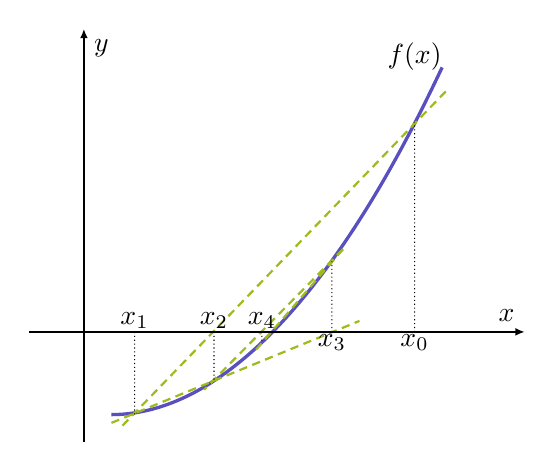
\begin{tikzpicture}[scale=7]
%
% Koordinater 
% ------------------------------------------------------
\coordinate (a) at (0.05,-0.05);
\coordinate (b) at (0.65,0.58);
\coordinate (c) at (0.6,0.48);		% x_0
\coordinate (d) at (0.07,-0.07);	% a
\coordinate (e) at (0.66,0.54); 	% b
\coordinate (f) at (0.092,-0.05);	% x_1
\coordinate (g) at (0.236,0.01);	% x_2
\coordinate (h) at (0.05,-0.065);	% a
\coordinate (i) at (0.5,0.12);		% b
\coordinate (j) at (0.45,0.228);	% x_3
\coordinate (k) at (0.47,0.25);		% a
\coordinate (l) at (0.218,-0.005);  % b
\coordinate (m) at (0.323,0.083);   % x_4
\coordinate (n) at (0.47,0.25);		% a
\coordinate (o) at (0.31,0.065);  % b
\coordinate (p) at (0.323,0.083);   % x_5
%
%        
% Streger 
% -------------------------------------------------------
  \draw[very thick, color=AAUblue2](a) parabola (b);
   
  \draw[densely dashed, thick, color = AAUgreen](d) -- (e); 
  \draw[densely dashed, thick, color = AAUgreen](h) -- (i); 
  \draw[densely dashed, thick, color = AAUgreen](k) -- (l);
  \draw[densely dashed, thick, color = AAUgreen](n) -- (o);   
%
% Punkter
% -------------------------------------------------------
%
  \node at (0.6,0.6) (){$f(x)$};
  
  \node at (0.6,0.08) (){$x_0$};
  \draw[densely dotted](0.6,0.1) -- (c);
  \node at (0.092,0.12) (){$x_1$}; 
  \draw[densely dotted](0.092,0.1) -- (f);
  \node at (0.236,0.12) (){$x_2$}; 
  \draw[densely dotted](0.236,0.1) -- (g);
  \node at (0.45,0.08) (){$x_3$}; 
  \draw[densely dotted](0.45,0.1) -- (j);
  \node at (0.323,0.12) (){$x_4$}; 
  \draw[densely dotted](0.323,0.1) -- (m);
%
%
% Koordinatsystemet 
% -------------------------------------------------------
\draw[thick,->] (-0.1,0.1) -- (0.8,0.1) node[anchor=south east]{$x$};
\draw[thick,->] (0,-0.1) -- (0,0.65) node[anchor=north west]{$y$};
%
\end{tikzpicture}
\end{center}
\end{frame}
\begin{frame}{Opgave 4: Den adaptive metode}
    Vi skal nu se på en anvendelse. Vi definerer en funktion ved
    \begin{align}
    f(x)=\left \{ \substack{-(x-\sqrt{2})^2 \text{  } \text{for} \text{  } x \leq \sqrt{2} \\ (x-\sqrt{2})^2\text{  } \text{for} \text{  } x > \sqrt{2}}
    \end{align}
    
    %Noget galt i ovenstående?
    
    Vi vil se på approksimation af integralet 
    \begin{align}
    \int_{0}^{3}f(x)dx    
    \end{align}
    % 
\end{frame}


\begin{frame}{Den adaptive metode}
    \begin{itemize}
        \item (a) Lav en Python funktion til beregning af funktionen defineret i (1).
        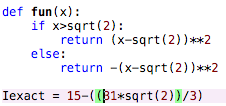
\includegraphics[]{Billeder/1.4(a).png}
    \end{itemize}
\end{frame}


\begin{frame}{Den adaptive metode}
    \begin{itemize}
        \item (b) Vis, at den eksakte værdi af integralet er $15-\frac{31\sqrt{2}}{3}$.
        \item \begin{align*}
            \int^{\sqrt{2}}_0-(x-\sqrt{2})^2+\int^3_{\sqrt{2}}(x-\sqrt{2})^2=15-\frac{29\sqrt{2}}{3}-\frac{2^{\frac{3}{2}}}{3}=15-\frac{31\sqrt{2}}{3} 
            \end{align*} \\
            Ved at tage integralet for begge funktioner, og derefter plusse dem sammen, fås den eksakte værdi $15-\frac{31\sqrt{2}}{3}$\\\\
    \end{itemize}
\end{frame}


\begin{frame}{Den adaptive metode}
    \begin{itemize}
        \item (c) Bestem integralet numerisk ved hjælp af de tre sammensatte kvadraturregler (midtpunkt, Trapez og Simpson). 
        Hvor mange ækvidistante inddelinger skal anvendes i hvert af de tre tilfælde for at opnå en fejl på mindre end $10^{-8}$?
        \item Ved Midtpunkt er fejlen mindre end $10^{-8}$ ved cirka $4096$ indelinger.\\
        Ved trapez sker dette først ved cirka $8192$, altså senere end ved midtpunkt.\\ 
        Ved Simpsonreglen sker dette ved ca $512$ og denne opnår dermed højere præcision ved færre iterationer end de foregående to.
    \end{itemize} 
\end{frame}


\begin{frame}{Den adaptive metode}
    \begin{itemize}
        \item (d) Lav i de tre tilfælde numeriske eksperimenter, baseret på fordobling af antal delepunkter, og brug dem til en eksperimentel bestemmelse af ordenen af de tre metoder. 
        Stemmer resultaterne med teorien? Hvis der er afvigelser, hvordan kan
        de så forklares?
        %Hvorfor springer orden så meget i Simpson efter 8192?
        \item For både trapez samt midtpunktreglen stabliseres der omkring en orden på $4$ efter et passende antal inddelinger hvilket stemmer overens med teorien, dette er dog ikke tilfældet for Simpson. Den opnår de $16$, men falder drastisk efterfølgende.
    \end{itemize}
\end{frame}


\begin{frame}{Den adaptive metode}
    \begin{itemize}
        \item (e) Prøv at anvende en simpel adaptiv metode til at bestemme integralet (2). 
        Hvad sker der, hvis man inddeler i to delintervaller af samme længde. 
        Hvordan bidrager de hver til fejlen i approksimationen? 
        Angiv resultaterne for både trapezreglen og Simpsons regel.
        %Vi har svært ved at skulle dele i to delintervaller og alt det Python-fis
        \item For simpsons adaptiv: Integralet af funktionen fra $1.5$ til $3$ er præcist, idet antallet af inddelinger er ligegyldigt, da det er et tredjegradspolynomium og funktionen forbliver stabil i hele intervallet. 
        Derimod sker der fra $0$ til $1.5$ det, at funktionen skifter og der er derfor behov for et større antal inddelinger. 
        Det biddrager hermed til, at denne del af aproksimationen giver en større fejl med behov for et større antal inddelinger.
        \item For Trapez: her biddrager begge intervaller lige meget til fejlen og kræver samme antal underindelinger(512 hvis mit bud om faktor 3 er korrekt) dette skyldes at præcisionen er mindre her hvorfor approskismationen ikke er lig funktionsværdien i intervallet fra 1.5 til 3 heller.
    \end{itemize}
\end{frame}
\section{Del 2: Numerisk løsning af differentialligninger}
\begin{frame}
\centering
\Huge
Del 2: \\
Numerisk løsning af differentialligninger
\end{frame}
%
\begin{frame}{Opgave 1: Lagrange-interpolation}
    Gennemgå teorien for Lagrange interpolation baseret på datapunkterne $x_0, \ldots, x_N$ og $f_0, f_1, \ldots , f_N$. 
\end{frame}

\begin{frame}{Lagrange-interpolation}
    \begin{itemize}
        \item Lagrange-interpolation handler om at finde et polynomium $p(x_k)=f(x_k)$ af mindst mulig grad og er således en måde at approksimere en funktionsværdi givet $x_0 \ldots x_N$ og $N+1 $  $y$ værdier.
        Det ønskes således at finde et polynomium med interpolationsegenskaben $p_{x_j}=y_j$,$j=0,1,\ldots,N$.

        \item Problemet omhandler således at finde et $N$'te grads polynomium $p$, der tager funktionsværdien for $f$ i en givet mængde punkter. 
        Ideen kan således relateres til taylorserier og konstruktion af taylorpolynomier, da disse ligeledes antager funktionsværdien i et givet udviklingspunkt.
    \end{itemize}
\end{frame}
\begin{frame}{Lagrange-interpolation}
    \begin{itemize}
        \item Lagrange-polynomier er defineret ved \\
            $
            l_k(x)=\frac{\prod_{\substack{j=0 \\ {j \neq k}}}^{N}(x-x_j)}{\prod_{\substack{j=0 \\ {j \neq k}}}^{N}(x_k-x_j)}=\frac{(x-x_0) \cdots (x-x_{j-1}) \cdot (x-x_{j+1})\cdots(x-x_N)}{(x_j-x_0)\cdots (x_j-x_{j-1}) \cdot (x_j-x_{j+1})\cdots (x_j - x_N)}
            $
        \item Et Lagrange-interpoleret andensgradspolynomium er således givet ved $ p(x)=f(x_0)\frac{(x-x_1)(x-x_2)}{(x_0-x_1)(x_0-x_2)}+f(x_1)\frac{(x-x_0)(x-x_2)}{(x_1-x_0)(x_1-x_2)}+f(x_2)\frac{(x-x_0)(x-x_1)}{(x_2-x_0)(x_2-x_1)} $
        \item Der eksisterer et entydigt Lagrange interpoleret polynomium for punkter givet ved $x_0, \ldots, x_N$ og $f_0, f_1, \ldots , f_N$.
        
    \end{itemize}
\end{frame}
\begin{frame}{Lagrange-interpolation bevis for entydighed}
    Ved at finde sådanne polynomier, er deres eksistens bevist. 
    Deres entydighed vil nu bevises. 
    Antag, at $q_n$ og $p_n$ er to forskellige polynomier med grad $\leq n$, og at de begge interpolerer samme data. 
    Så er graden af polynomiet $p_n - q_n$ også $\leq n$, og værdien af dette polynomie er $0$ ved $n+1$ datapunkter. 
    Men en polynomie med grad $n$ har højst $n$ nuller, medmindre det er nulpolynomiet. 
    Således er $p_n - q_n = 0$, hvormed $p_n = q_n$. 
\end{frame}

%HER DANIEL
\begin{frame}
\frametitle{Modificeret Euler metode og \phantom{HHHHHHH} trapezmetoden}
\begin{itemize}
\item Modificeret Euler metode anvendt på $$\frac{dy}{dx}=f(x),\phantom{hi}y(a)=y_0$$
\item Trapezmetoden anvendt på $$y_0 + \int_a^b f(x) dx$$
\end{itemize}
\end{frame}
%
\begin{frame}
\frametitle{Modificeret Euler metode og \phantom{HHHHHHH} trapezmetoden}
\begin{itemize}
\item For modificeret Euler metode
\begin{align*}
x_{n+1} &= x_n + h\\
k_1 &= f(x_n)\\
k_2 &= f(x_{n+1} )\\
y_{n+1} &= y_n + \frac{h}{2}(k_1 + k_2)\\
&\downarrow\\
y_N &= y_0 + \frac{h}{2}\left( f(x_0) + 2(f(x_1) + \cdots + f(x_{N-1})) + f(x_N) ) \right)\\
 &= y_0 + \frac{h}{2}\left(f(a) + 2\sum_{j=1}^{N-1}f(x_j) + f(b)\right)
\end{align*}
\end{itemize}
\end{frame}
%
\begin{frame}
\frametitle{Modificeret Euler metode og \phantom{HHHHHHH} trapezmetoden}
\begin{itemize}
\item For trapezmetoden
\begin{align*}
T_N &= \frac{h}{2} \left(f(a) + 2\sum_{j=1}^{N-1} f(x_j) + f(b) \right)\\
y_0 + T_N  &= y_0 + \frac{h}{2} \left(f(a) + 2\sum_{j=1}^{N-1} f(x_j) + f(b) \right)
\end{align*}
\end{itemize}
\end{frame}
\subsection{Numerisk eksperiment}
\begin{frame}{Definition af funktion}
    Vi definerer funktionen $f$ ved
    \begin{align*}
    f(x)=x^2-\sin(10x), x \in \mathbb{R}
    \end{align*}
    Vi ser på intervallet $\left [0,3 \right ]$ og definerer punkterne $x_j = \frac{3j}{N}, j = 0, 1, \ldots, N$, så at vi har $N+1$ ækvidistante punkter. Vi definerer også $f_j=f(x_j), j=0,1,\ldots,N.$ Vi betegner med $p_N$ det interpolerende polynomium baseret på disse data.  
\end{frame}
%\begin{frame}{Opgave 3: Fejl}
%    Scriptet \textsc{Interpolation bin.py} giver en vurdering af den maksimale fejl 
%    \begin{align*}
%    \underset{x \in \left [0,3 \right ]}{\text{max}} \lvert f(x)-p_N(x) \rvert
%    \end{align*}
%    for forskellige værdier af $N$. Det beregner også en teoretisk vurdering af fejlen, se nedenfor. Gennemgå dette script i detaljer. \textbf{Bemærk} at dette script ikke bruger \textsc{numpy}, men er baseret på lister. Begrundelsen er at vi skal være i stand til at modificere dette script til at anvende \textsc{decimal modulet}. Efter gennemgangen skal I modificere scriptet til at generere plots for små værdier af $N$, der i samme figur viser grafen for $f(x)$, grafen for $p(x)$ og knudepunkterne.
%\end{frame}

\begin{frame}{Gennemgang af scriptet}
    \begin{itemize}
        \item Definition af Lagrange funktionen
        \item Lav et Lagrange-interpoleret polynomium. 
        \item \textsc{Interpolation bin funktioner.py}, er  modificeret til den genererer plots. 
    \end{itemize}
    \begin{align*}
    \underset{x \in \left [0,3 \right ]}{\text{max}} \lvert f(x)-p_N(x) \rvert
    \end{align*}
\end{frame}

%MANGLER BILLEDE!
%\begin{frame}
%\frametitle{Eulers metode og RK4}
%\begin{itemize}
%\item Python
%\end{itemize}
%\end{frame}
\begin{frame}
\frametitle{Betydning af parametrene}
\begin{itemize}
\item Fordobling af $\alpha$
\end{itemize}

\begin{minipage}{0.49\textwidth}
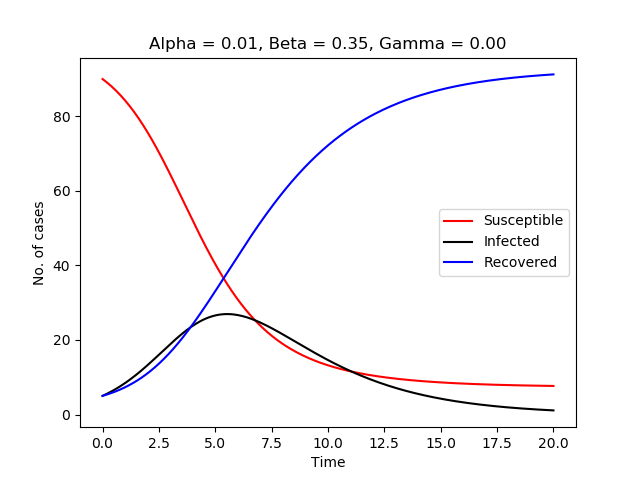
\includegraphics[scale=0.3]{fig/img/t_a1_b35_g0.png}
\end{minipage}
%
\begin{minipage}{0.49\textwidth}
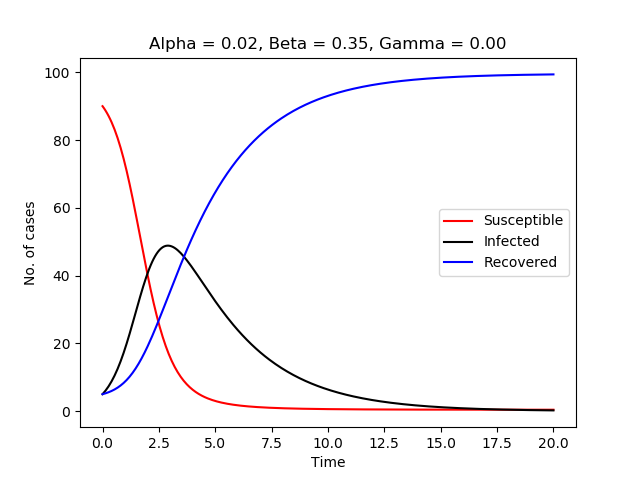
\includegraphics[scale=0.3]{fig/img/t_a2_b35_g0.png}
\end{minipage}
\end{frame}
%
\begin{frame}
\frametitle{Betydning af parametrene}
\begin{itemize}
\item Fordobling af $\beta$
\end{itemize}

\begin{minipage}{0.49\textwidth}
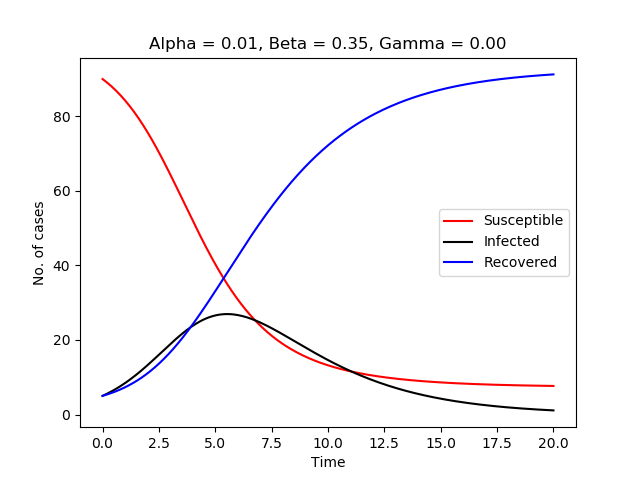
\includegraphics[scale=0.3]{fig/img/t_a1_b35_g0.png}
\end{minipage}
%
\begin{minipage}{0.49\textwidth}
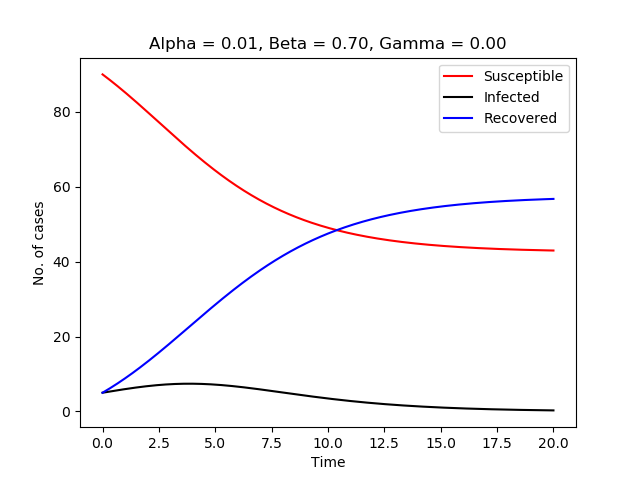
\includegraphics[scale=0.3]{fig/img/t_a1_b7_g0.png}
\end{minipage}
\end{frame}
%
\begin{frame}
\frametitle{Betydning af parametrene}
\begin{itemize}
\item Fordobling af antal immune, 
\item $x_{1,0}$ fra 90 til 85
\end{itemize}

\begin{minipage}{0.49\textwidth}
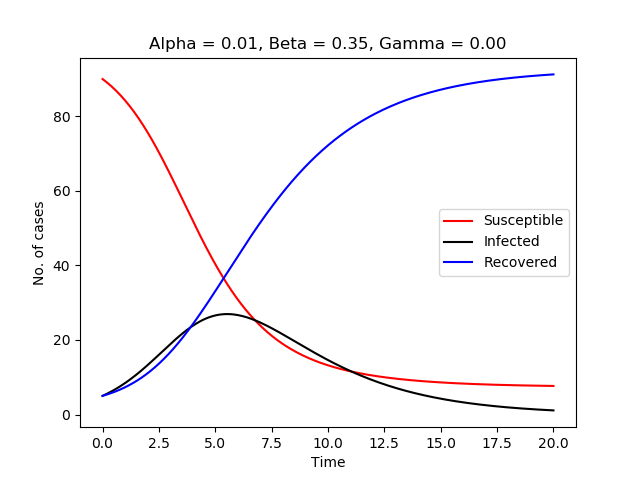
\includegraphics[scale=0.3]{fig/img/t_a1_b35_g0.png}
\end{minipage}
%
\begin{minipage}{0.49\textwidth}
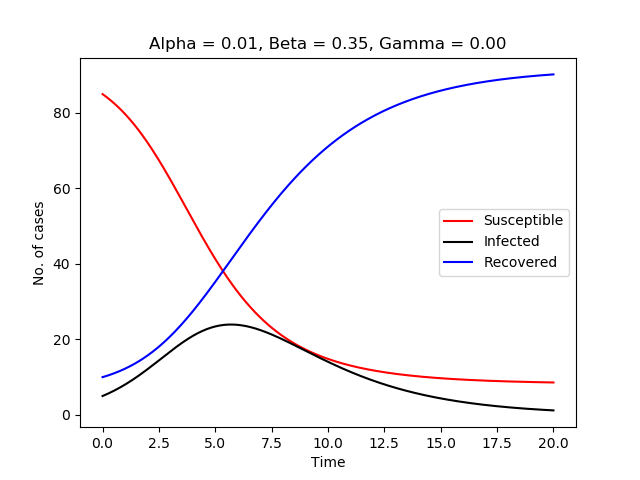
\includegraphics[scale=0.3]{fig/img/t_x1_5_x2_85.png}
\end{minipage}
\end{frame}
%
\begin{frame}
\frametitle{Betydning af parametrene}
\begin{itemize}
\item Ændring af indledende syge, $x_{2,0}$, fra $5$ til $1$
\end{itemize}

\begin{minipage}{0.49\textwidth}
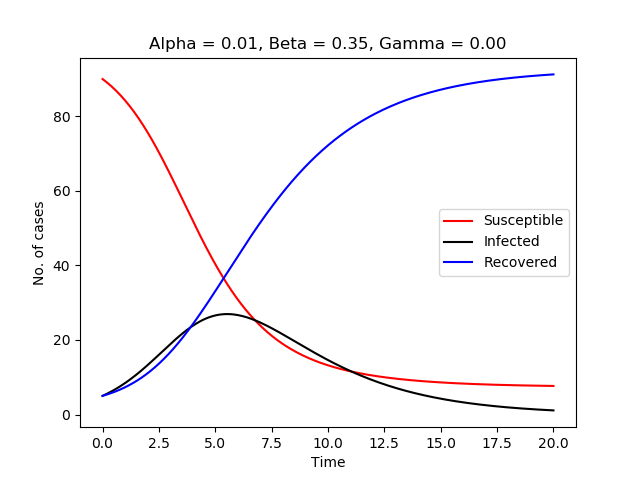
\includegraphics[scale=0.3]{fig/img/t_a1_b35_g0.png}
\end{minipage}
%
\begin{minipage}{0.49\textwidth}
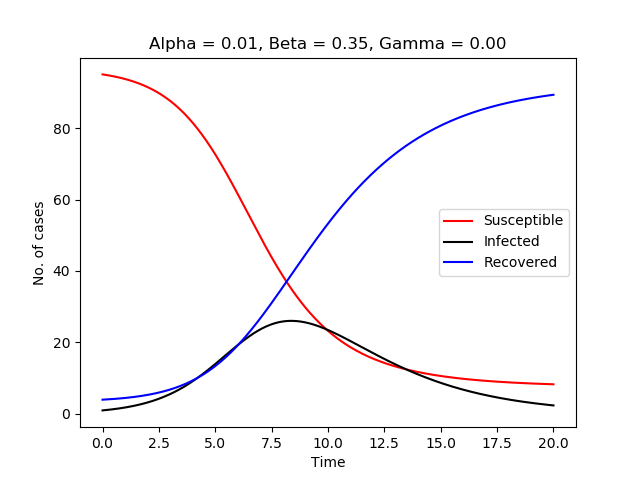
\includegraphics[scale=0.3]{fig/img/t_x1_1_x2_95.png}
\end{minipage}
\end{frame}
%


\begin{frame}
\frametitle{Vaccine Indførelse}
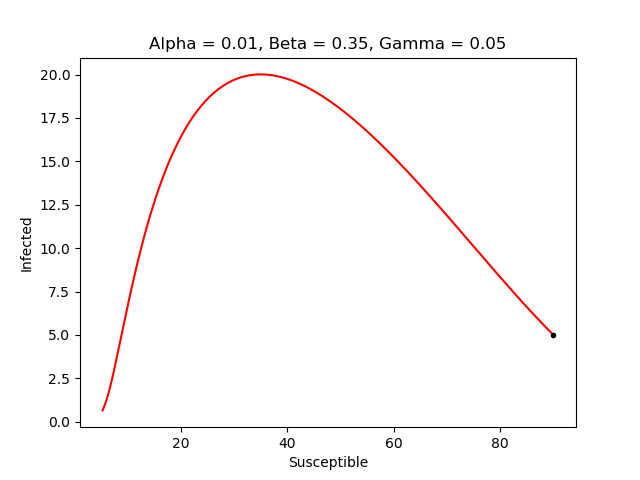
\includegraphics[scale=0.295]{img/a1_b35_g5.png}
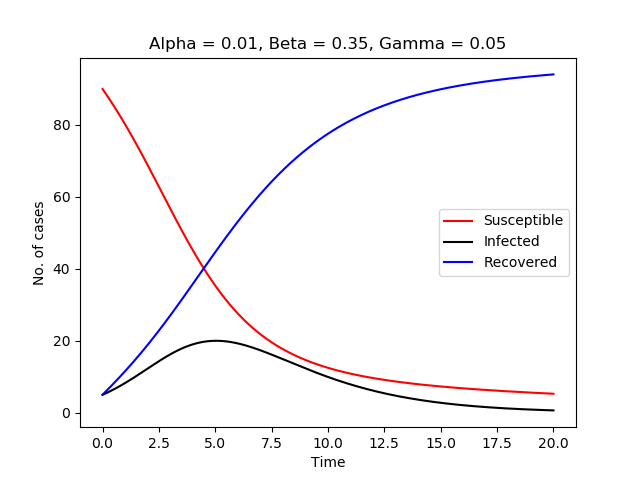
\includegraphics[scale=0.295]{img/t_a1_b35_g5.png}
\end{frame}
%
\begin{frame}
\frametitle{Vaccine Indførelse}
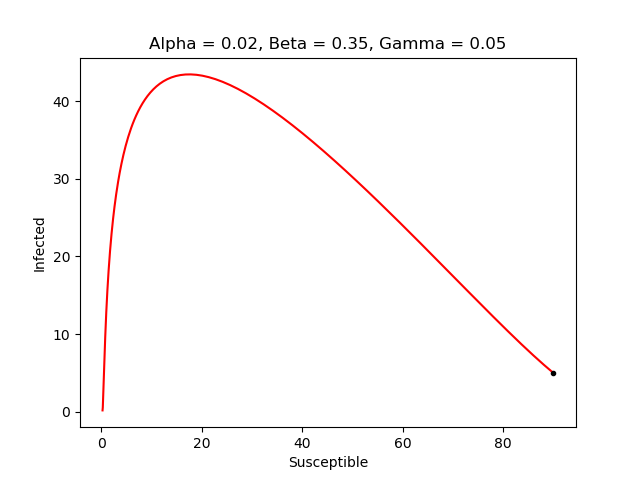
\includegraphics[scale=0.295]{img/a2_b35_g5.png}
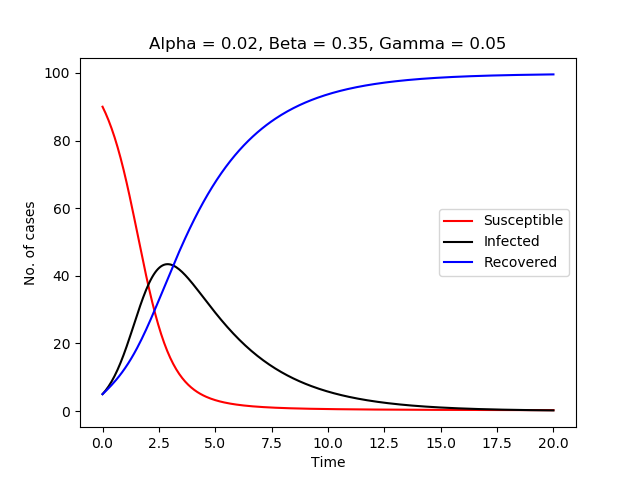
\includegraphics[scale=0.295]{img/t_a2_b35_g5.png}
\end{frame}


\bibliographystyle{apalike}
\nocite{*}
% \begin{frame}{References}
% \tiny\bibliography{bib/bibliography}
% \end{frame}

\end{document}